\documentclass[notitlepage]{article}
\usepackage[utf8]{inputenc} 
\usepackage{geometry} 		
\usepackage{chngcntr}
\usepackage{amsmath} 			
\usepackage{amssymb}			
\usepackage{mathtools}		
\usepackage{comment} 			
\usepackage{mdframed}			
\usepackage{xcolor}				
\usepackage{fancyhdr}			
\usepackage{listings}			
\usepackage{color}				
\usepackage{tikz}	
\usepackage{tasks}			
\usepackage{exsheets}	
\usepackage{blindtext}	
\usepackage{array}			
\usepackage{empheq}
\usepackage{caption}
\usepackage{pdfpages}
\usepackage{tabularx}
\usepackage{lscape}

\geometry{ 						%Format titlepage (interrupted by newgeometry)
	a4paper,
	total={170mm,257mm}%,
	%left=0mm,
	%top=0mm,
}

%START DEFINE YOUR VARIABLES HERE

\newcommand{\documentName}{Software Design Specification}
\newcommand{\projectName}{Label Refinement by Behavioral Similarity}

%END DEFINE YOUR VARIABLES HERE

\title{%
	\documentName\text{ } \\
  \large \projectName\text{ } \\
  }

\author{
	\large \underline{Document owners:}\\ 
	Bianka Bakullari\\
	\texttt{}
	Christopher Beine\\
	\texttt{}
	Nicole Ventsch\\
	\texttt{}
	Juan Garza\\
	\texttt{}
}

\date{\small{Last edited: \today}}

\pagestyle{fancy}
\fancyhf{}
\rhead{}
\lhead{\documentName\space-\space\projectName}

\makeatletter					%Prefix to add ToC to titlepage
\newcommand*{\toccontents}{\@starttoc{toc}}
\renewcommand*\contentsname{}
\makeatother
                  

\begin{document}

\begin{titlepage}
\clearpage\maketitle			%Clear title page
\thispagestyle{fancy}
\tableofcontents
\end{titlepage}

\rfoot{\thepage}				%Start printing page-numbers, after title page.

\newgeometry{ 					%Default page formatting on-going #1
	total={170mm,257mm},
	left=20mm,
	top=25mm,
    bottom=30mm					%Causes warning
}

\begin{flushleft}				%Default page formatting on-going #2


\section{Introduction}
\subsection{System Overview}
\subsection{Design Map}
\subsection{Supporting Materials}
\subsection{Definitions and Acronyms}

\section{Design Considerations}
\subsection{Assumptions and Dependencies}
\subsection{General Constraints}
\subsection{Goals and Guidelines}
\subsection{Development Methods}

\section{Architectural Strategies}

\subsection{Sotware}
As mentioned the Software is divided into two main Parts, the Front-end and Back-end.\\ 
\medskip
The Back-end will be implemented with Python.
Python is an popular and widely used language within the data data science. The language provides many libraries for data science like pm4py.
The webframwork Flask which is written in Python too, provides a fast applicaton deployment with a minimal usage of external libraries so that we can 
focus on the algorithm design. A User can Access the Back-end via an API which distributes the data to the required components.\\
\medskip
The Front-end will be implemented with JavaScript. We will use a minimalistic Model-View-Controller (MVC) approach. The Model only represents the data like 
the customization paramters for the algorithm or the event log file. The Model will be easily converted into a JSON Object, which can be evaluated by the backend.
The View represents the User Interface markup and is written in HTML5. Logic implementation is not required in the View part. The Controller part represents 
the business logic. Since the front-end acts as a of abstraction layer for our Back-end API, the Controller should be as small as possible.\\
\medskip
A database system is not set up, since the project focus is the refining algorithm. However the applicatoins will keep track of the five last uploaded files and 
their refined event logs. For this we will use the server file system. 

\subsection{Enhancements}
In order to realise a future development following measure will be implemented.

Using the \textit{abstract class} in combinadtion with the \textit{factory} pattern to exchange important software and algorithms components. 
This will be implemented for the file conversion, file creation or cost function. Additional functionality has to implement a given interface which will be registerd 
to a factory methode afterwards. Additional code is not required. 

Developing an API which can be included into other system or workflow. The event log refinement can included into other applicatons. 
Individual components can be exchanged more easily 

\section{System Architecture}
The following UML displays the main application components and where they are deployed. The final application will be deployed on an application server which the user can access over an internet browser on his own machine. Therefore the system is independent of the users operating system. There are two option to perform the 
algorithm:

\begin{itemize}
	\item The user can access the JavaScript Front-end application via HTTP which provides an user friendly UI. There the user can set all required parameters and send them to the API.
	\item Additional, the user can access the API directly via HTTP with the required parameter. So the application can integrate into other application which could be helpful to perform preprocessing steps or to use the refined labels in another application. .
\end{itemize}




\includegraphics[scale=0.4]{"Architecture Overview".png}

\subsection{Client Machine}
The Client Machine is just a device with internet connection. It is not directly part of the application but is required to access to functionality.
To use the User Webinterface a Google Chrome or Mozilla Firefox Browser is required. The Client does not need a special operating system or system structure to user 
the project application.
\subsection{Front-end}
The Front-end provides the User Interface for a simple application access. It is created with HTML5 and JavaScript and redirects the User inputs to API.
So the end user must not know the API interface, required data formats and protocols.
\subsection{Refining Label API}
The Refining Label API is the main access point for the refining algorithm. Every communication goes through this API. After sending data, 
the API will validate them, execute some preprocessing steps like file conversion and finally execute the refining algorithm and returning the result to the calling user or system. 
Additional the API acts as a connection between the other Modules. Is connects the user access, algorithm and file handling.
Therefore each of the other components is independent and low coupling and high cohesion is achieved   
\subsection{File Store}
The File Store is an abstraction layer for the servers file system. It will keep track on the updates files and offers functions to store 
refined XES files on the server. It also monitors the memory utilization.
\subsection{Refining Event Labels}
The Refining Event Label components is responsible for the final refining algorithm. 
It contains functionality to calculate costs, execute preprocessing steps, horizontal clustering of variants and the vertical refinement.
To offer a maintainable and extensible system this component will provides interfaces to exchange mentioned functionalities. 
The following subcomponents exist: 


\subsection{Event Log Converter}
The Event Log Converter is a Framework to convert different files types into an Event Log and convert them back into files. 
For our project the system provides functionality for XES and CSV import and export. 
The Framework can easily be extended with additional file types without changing the core functionality.
\medskip
The following UML class diagram display the Framework structure:

\begin{landscape}
\includegraphics[width=\columnwidth]{"Event Log Converter CD".png}
\end{landscape}
The FileUtility provides access to the framework and its functionality.
The functions \textit{create\_file(eventLog: EventLog, type:string): string} realises the XES and CSV file uploader requirement and 
the \textit{get\_event\_log\_from\_file(string path): string} realises the Download refined XES event log file requirement. 

The Factory and Abstract Class Pattern provides the conversion of multiple file types with the same method. The Factory get the required file type as string and 
will return the corresponding Converter or Creator. Each file converter must implement the abstract class FileConverter and a file creator must implement
the abstract class FileCreator.\\
\medskip
If other file types should be supported by the application the developer only has to write another Creator/Converter for the type.
Via the \textit{registerImport(fileType:string, creator :FileCreator)} and \textit{registerExport(fileType:string, converter :FileConverter)} methods these classes can 
be injected in the FileUtility class. Afterwards the functionality is accessible in the whole application, additional code is not required.






\section{Policies and Tactics}


\subsection{Ensuring Requirements Realization}
To ensure the realization of all requirements specified in the Requirement Specification Document, the corresponding modules have to be designed.
The table below describes which modules are responsible for which requirement and which functionalities are used for the implementation of the module. \\

\medskip
%\newpage
\begin{tabularx}{\textwidth}{|p{6cm}|p{0.4cm}|p{4cm}|p{5cm}|}
\hline
\textbf{Requirements}
&\textbf{ID} 
&\textbf{Modules}
&\textbf{Functionalities}
\\
\hline
-Upload CSV event log file.
\newline -Upload XES event log file.
&
5
\newline 6
&
1.1 File converter.
\newline 1.2 Preprocessing log.
& 
1.1.1 getEventLogFromFile() 
\newline 1.1.2 readXES()
\newline 1.2.1 checkEventLog() 
\newline 1.2.2 createlookUpTable()
\newline 1.2.3 getVariants() \\
\hline
-Customize threshold for cost function.
\newline -Customize horizontal threshold.
\newline -Customize vertical threshold.
\newline -Choose set of imprecise labels.
&
7
\newline 8
\newline 9
\newline 10
&
2. Customize.
&
2.1 setCandidates()
\newline 2.2 getCandidates()
\newline 2.3 setVerticalThreshold()
\newline 2.4 getVerticalThreshold()
\newline 2.5 setHorizontalThreshold()
\newline 2.6 getHorizontalThreshold()
\\
\hline
-Calculate costs
- \textcolor{red}{Probably is a good idea to have an optimalMatching() function that gets as a parameters the set of possible mappings (i.e. from the mappings() function) and returns an object with the best mapping and its cost. Then we project that cost directly to the edges of the graph instead of storing them in the symmetric matrix (i.e. costMatrix()) in this way we save memory space.}
&
1
&
3. Cost function.
&
3.1 mappings()
\newline 3.2 costMapping()
\newline 3.3 costMatrix()
\newline 3.4 updateGraph()
\\ 
\hline
-Clustering of traces
\newline -Refine labels horizontally across traces.
&
2
\newline 3 
&
4. Horizontal clustering of variants.
&
4.1 clusterDetection()
\newline 4.2 horizontalRefinement()
	\\ 
\hline
-Refine labels vertically within traces.
&
4
&
5. Vertical refinement.
&
5.1 verticalRefinement()
	\\ 
\hline
$- -$
&

&
6. Post-Processing.
&
6.1 updateLookUpTable()
\newline 6.2 updateEventLog()	\\ 
\hline
-Download refined XES event log file.
&
11
&
7. File Creator.
&
6.1 createFile()
\newline 6.2 storeFile()
\\ 
\hline
\end{tabularx} \\

\medskip

A detailed description of the modules and functionalities is given in Section 6.



















\section{Detailed System Design}
The main algorithm ``Refining Event Labels" will be split up into multiple modules that contain the main parts of the algorithm according to chapter 5.1. These modules will be explained in detail in the following subsections.
\subsection{Module 1.1: File Converter}
\textit{Name}: File Creator

\textit{Related Component}: Event Log Converter.

\textit{Type}: module.

\textit{Description}: This module is responsible for creating a table from the data the user uploads. The event log provided by the user is read and stored internally containing all the original columns. 

\textit{Attributes}: none.

\textit{Resources}: none.

\textit{Operations}: 
\medskip

\par
\begingroup
\leftskip4em
\textbf{1.1.1}

\textit{Name}: getEventLogFromFile()

\textit{Arguments}: path to a log file in CSV format or XES format.

\textit{Returns}: event log in XES format.

\textit{Description}: the file from the path which the user submits is read and stored in XES format. In case the file is originally in CSV format, the file is first converted to XES format and then stored.

\textit{Precondition}: the path provided by the user leads to a CSV file or an XES file.

\textit{Postcondition}: the table is stored internally as an XES file.

\textit{Exceptions}: none.
\par
\endgroup

\medskip

\par
\begingroup
\leftskip4em
\textbf{1.1.2}

\textit{Name}: readXES()

\textit{Arguments}: a file in XES format.

\textit{Returns}: an event log object.

\textit{Description}: the XES file is read and stored as an event log object.

\textit{Precondition}: an XES file was created using getEventLogFromFile().

\textit{Postcondition}: an event log object is created and stored internally.

\textit{Exceptions}: none.
\par
\endgroup

\medskip

\subsection{Module 1.2: Preprocessing Log}
\textit{Name}: Preprocessing Log.

\textit{Related Component}: Refining Event Labels.

\textit{Type}: module.

\textit{Description}: this module is responsible for preprocessing the data. The file provided by the user is verified, that is, if it has the right standard format, otherwise an error is thrown. Moreover, a table containing all unique traces (i.e. variants) and the list of IDs corresponding to these traces is created.

\textit{Attributes}: none.

\textit{Resources}: none.

\textit{Operations: }
\medskip


\par
\begingroup
\leftskip4em
\textbf{1.2.1} 

\textit{Name}: checkEventLog()

\textit{Arguments}: an event log object obtained from readXES().

\textit{Returns}: Boolean (True or False).

\textit{Description}: verify it the event log object has the standard format, i.e., whether it contains an activity column, an ID column and a time stamp column. If these attributes are present in the object, ``True" will be returned, otherwise ``False" will be returned. 

\textit{Precondition}: an event log object was created using readXES().

\textit{Postcondition}: if ``True" is returned, the event log object is contains all the required attributes, otherwise an error will be displayed.

\textit{Exceptions}: none.
\par
\endgroup

\medskip

\par
\begingroup
\leftskip4em
\textbf{1.2.2}

\textit{Name}: lookupTable()

\textit{Arguments}: an event log object.

\textit{Returns}: lookup table containing a ``variants" column and an ``ID" column.

\textit{Description}: the variants are extracted from the event log object and serve as key in the lookup table. The values for each key in the lookup table correspond to the IDs of the traces that belong to a particular variant. The variants are stored as arrays and the corresponding IDs as a list.

\textit{Precondition}: an already verified event log object.

\textit{Postcondition}: a lookup table is stored containing the variants and IDs corresponding to those variants.

\textit{Exceptions}: none.

\par
\endgroup

\medskip

\par
\begingroup
\leftskip4em
\textbf{1.2.3}

\textit{Name}: getVariants()

\textit{Arguments}: a lookup table obtained from lookupTable().

\textit{Returns}: set of unique trace variants.

\textit{Description}: a set containing all the variants is created for further computations (mappings). Here, it is not mandatory to have directly access to the IDs.

\textit{Precondition}: a non empty lookup table.

\textit{Postcondition}: a non empty set containing the arrays describing each variant.

\textit{Exceptions}: none.

\par
\endgroup

\subsection{Module 2: Customize}
\textit{Name}: Customize.

\textit{Related Component}: Refining Event Labels.

\textit{Type}: module.

\textit{Description}: this module is responsible to customize the algorithm parameters. The module serves as a model class and it is passed as an argument to the refining algorithm.
It stores information about the candidates to refine and the vertical and horizontal threshold. It also automatically validates these parameters.  

\textit{Attributes}: none.

\textit{Resources}: none.

\textit{Operations}: 
\medskip


\par
\begingroup
\leftskip4em
\textbf{2.1} 

\textit{Name}: setCandidates()

\textit{Arguments}: traces for which should be refined.

\textit{Returns}: void.

\textit{Description}: store the traces which are ''imprecise" according to the user expertise. 

\textit{Precondition}: valid trace model.

\textit{Postcondition}: traces are stored in the model.

\textit{Exceptions}: none.

\par
\endgroup

\medskip


\par
\begingroup
\leftskip4em
\textbf{2.2} 

\textit{Name}: getCandidates()

\textit{Arguments}: none.

\textit{Returns}: a list of traces.

\textit{Description}: obtain the traces which are ''imprecise" according to the user expertise. 

\textit{Precondition}: none.

\textit{Postcondition}: none.

\textit{Exceptions}: none.
\par
\endgroup

\par
\begingroup
\leftskip4em
\textbf{2.3} 

\textit{Name}: setVerticalThreshold()

\textit{Arguments}: vertical threshold as floating point value.

\textit{Returns}: void.

\textit{Description}: store the threshold for the vertical refinement. Values bigger than 1 are converted to 0.99 and values smaller than 0 are converted to 0.1

\textit{Precondition}: none.

\textit{Postcondition}: none.

\textit{Exceptions}: none.
\par
\endgroup


\par
\begingroup
\leftskip4em
\textbf{2.4} 

\textit{Name}: getVerticalThreshold()

\textit{Arguments}: none.

\textit{Returns}: vertical threshold as floating point value.

\textit{Description}: obtain the vertical threshold.

\textit{Precondition}: none.

\textit{Postcondition}: none.

\textit{Exceptions}: none.
\par
\endgroup



\par
\begingroup
\leftskip4em
\textbf{2.5} 

\textit{Name}: setHorizontalThreshold()

\textit{Arguments}: horizontal threshold as floating point value.

\textit{Returns}: void.

\textit{Description}: store the threshold for the horizontal refinement. Values bigger than 1 are converted to 0.99 and values smaller than 0 are converted to 0.1

\textit{Precondition}: none.

\textit{Postcondition}: none.

\textit{Exceptions}: none.
\par
\endgroup


\par
\begingroup
\leftskip4em
\textbf{2.6} 

\textit{Name}: getHorizontalThreshold()

\textit{Arguments}: none.

\textit{Returns}: horizontal threshold as floating point value.

\textit{Description}: obtain the horizontal threshold.

\textit{Precondition}: none.

\textit{Postcondition}: none.

\textit{Exceptions}: none.
\par
\endgroup


\subsection{Module 3: Cost function}
\textit{Name}: Cost function.

\textit{Related Component}: Refining Event Labels.

\textit{Type}: module.

\textit{Description}: this module is responsible for calculating the costs of all mappings between each pair of variants and selecting the optimal mapping with the least costs. 

\textit{Attributes}: none.

\textit{Resources}: the weights used for the calculation of costs.

\textit{Operations}: 
\medskip

\par
\begingroup
\leftskip4em
\textbf{3.1} 

\textit{Name}: mappings()

\textit{Arguments}: two distinct trace variants.

\textit{Returns}: a set of possible mappings.

\textit{Description}: for each pair of variants the set of common activity labels occurring in both variants is obtained. If this set is empty, no mapping is possible. Otherwise, if none of the common labels appears more than once in any of the variants, the unique mapping is yielded. In the other case, all combinations of possible mappings are yielded as a set where each mapping is an array of pairs of the positions that were matched together.

\textit{Precondition}: iterate over all pairs of trace variants obtained from getVariants().

\textit{Postcondition}: for each mapping, the cost function is computed.

\textit{Exceptions}: none.
\par
\endgroup


\medskip

\par
\begingroup
\leftskip4em
\textbf{3.2} 

\textit{Name}: costMapping()

\textit{Arguments}: two trace variants and a mapping between them.

\textit{Returns}: the cost of the mapping as a floating point value.

\textit{Description}: for each pair in the mapping, the number of distinct predecessors and successors and the distances to other matched pairs is counted. Then, a final sum is computed by considering these costs for all matched pairs and also the number of unmatched labels appearing in both traces. Note that, each term is adjusted with a corresponding weight. Simultaneously all costs between pairs of variants are stored in a list so that the minimal one is chosen.

\textit{Precondition}:calculate the costs for each mapping yielded by mappings().

\textit{Postcondition}: for each mapping, the corresponding cost is computed.

\textit{Exceptions}: none.
\par
\endgroup


\medskip

\par
\begingroup
\leftskip4em
\textbf{3.3} 

\textit{Name}: costMatrix()

\textit{Arguments}: the cost of the optimal mapping for each pair of variants.

\textit{Returns}: a symmetrical 2-dimensional matrix.

\textit{Description}: The matrix contains 0s in the diagonal and the entry in position $[i][j]$ corresponds to the cost of the optimal mapping between variant $i$ and variant $j$. 

\textit{Precondition}: the cost of the optimal mapping between two variants is obtained by choosing the minimal entry in the list of costs of their possible mappings stored in costMapping().

\textit{Postcondition}: for each pair of variants, the cost of the optimal mapping is known.

\textit{Exceptions}: none.
\par
\endgroup


\medskip

\par
\begingroup
\leftskip4em
\textbf{3.4} 

\textit{Name}: updateGraph()

\textit{Arguments}: the cost of the optimal mapping for each pair of variants and the set of variants.

\textit{Returns}: an undirected weighted graph.

\textit{Description}: for each variant there is a set of vertices corresponding to the events occurring in the variant. Each edge only connects matched pairs and for the pairs being in the candidate set the weight of each edge corresponds to the cost of the optimal mapping. Otherwise the weight of the edge is 0.

\textit{Precondition}: the weights for the edges are obtained from the costMatrix().

\textit{Postcondition}: each variant has to be identified in the graph in order to perform the horizontal and vertical refinements in the next steps.

\textit{Exceptions}: none.
\par
\endgroup


\subsection{Module 4: Horizontal clustering of variants}
\textit{Name}: Label refinement based on clusters.

\textit{Related Component}: Refining Event Labels.

\textit{Type}: module.

\textit{Description}: this module clusters the event log and performs the label refinement based on these clusters.

\textit{Attributes}: \begin{itemize}
	\item Event log graph which should be refined.
	\item Customize object for the horizontal thresholds.
\end{itemize}

\textit{Resources}: none.

\textit{Operations}: 
\medskip

\par
\begingroup
\leftskip4em
\textbf{4.1} 

\textit{Name}: clusterDetection()

\textit{Arguments}: a graph and a customization Object (Module 2).

\textit{Returns}: a list of subgraphs.

\textit{Description}: group events in the same variant based on their similarity. Two events are considered to be in the same variant if their normalized cost is below the variant threshold $z_v$. this similarity is expressed by removing edges which cost is below $z_v$. As a result of removing these edges, a set of subgraphs is obtained and serve as cluster for the horizontal and vertical refinement. 

\textit{Precondition}: a complete undirected weighted graph generated from updateGraph().

\textit{Postcondition}: a list of undirected weighted subgraphs obtained from updateGraph().

\textit{Exceptions}: none.
\par
\endgroup

\medskip

\par
\begingroup
\leftskip4em
\textbf{4.2} 

\textit{Name}: horizontalRefinement()

\textit{Arguments}: a list of undirected weighted subgraphs and a customization Object (Module 2).

\textit{Returns}: void.

\textit{Description}: given the set of candidate labels, perform relabelling of events for each cluster of subgraphs, that is, give a new label to each of the events in the set of candidate labels. The relabelling is done exclusively in the graph.

\textit{Precondition}: a list of undirected weighted subgraphs obtained from clusterDetection().

\textit{Postcondition}: an updated list of undirected weighted subgraphs with new labels (horizontal refinement).

\textit{Exceptions}: none.
\par
\endgroup

\subsection{Module 5: Vertical Refinement}
\textit{Name}: Label refinement within variant.

\textit{Related Component}: Refining Event Labels.

\textit{Type}: module.

\textit{Description}: this module execute the label refinement within variant for the Event log and is part of the refinement algorithm.

\textit{Attributes}: none.

\textit{Resources}: none.

\textit{Operations}: 
\medskip

\par
\begingroup
\leftskip4em
\textbf{5.1} 

\textit{Name}: verticalRefinement()

\textit{Arguments}: a list of undirected weighted subgraphs and a customization Object (Module 2).

\textit{Returns}: void.

\textit{Description}: given the set of candidate labels and the unfolding threshold $v_f$, perform relabelling of events as indicated in the section 5.4 from \cite{paper}.

\textit{Precondition}: a list of undirected weighted subgraphs with horizontal refinement.

\textit{Postcondition}: an updated list of undirected weighted subgraphs with new labels (vertical refinement).

\textit{Exceptions}: none.
\par
\endgroup




\subsection{Module 6: Post-Processing}
\textit{Name}: Embed refinements into original log.

\textit{Related Component}: File converter.

\textit{Type}: module.

\textit{Description}: this module is responsible for executing the refinements in the log level. That is, update the original event log with refined labels.

\textit{Attributes}: the undirected weighted graph containing the new labels for each variant.

\textit{Resources}: the initial table describing the original event log.

\textit{Operations}: 
\medskip

\par
\begingroup
\leftskip4em
\textbf{6.1} 

\textit{Name}: updateLookUpTable()

\textit{Arguments}: an undirected weighted graph and the lookup table.

\textit{Returns}: an updated lookup table with refined labels.

\textit{Description}: replace each old variant in the lookup table with the new refined one.

\textit{Precondition}: unique case IDs.

\textit{Postcondition}: an updated lookup table.

\textit{Exceptions}: none.
\par
\endgroup


\medskip

\par
\begingroup
\leftskip4em
\textbf{6.2} 

\textit{Name}: updateEventLog() \textcolor{red}{Here, what is table referred to? The event log? I changed to updateEventLog() since we are using an event log object but feel free to make any changes :)}

\textit{Arguments}: an updated lookup table.

\textit{Returns}: an event log object with refined labels for the complete event log.

\textit{Description}: replace each old variant in the original event log object with the new refined one.

\textit{Precondition}: an updated lookup table.

\textit{Postcondition}: the updated event log object contains all original information from the event log but with the refined candidate labels.

\textit{Exceptions}: none.
\par
\endgroup




\subsection{Module 7: File Creator}
\textit{Name}: File Creator

\textit{Related Component}: Refining Event Labels / File Upload.

\textit{Type}: module.

\textit{Description}: utility class to export and store an event logs as a XES file.

\textit{Attributes}: an event log object.

\textit{Resources}: none.

\textit{Operations}: 
\medskip
\par
\begingroup
\leftskip4em
\textbf{6.1} 

\textit{Name}: createFile()

\textit{Arguments}: event log object.

\textit{Returns}: void.

\textit{Description}: converts the event logs a XES file.

\textit{Precondition}: a valid event log format.

\textit{Postcondition}: a XES file is created.

\textit{Exceptions}: none.
\par
\endgroup

\medskip
\par
\begingroup
\leftskip4em
\textbf{6.2} 

\textit{Name}: storeFile()

\textit{Arguments}: a directory path.

\textit{Returns}: the create file path.

\textit{Description}: stores the previous created file at given location.

\textit{Precondition}: a existing directory Path.

\textit{Postcondition}: the XES file is stored.

\textit{Exceptions}: NotADirectoryException
\par
\endgroup

\subsection{Uses/Interactions}
The components from the section System Architecture and the related modules result in the following System flow:\\

\begin{landscape}
	\newgeometry{
		total={250mm,210mm},
		left=0mm
	}
\includegraphics[width=297mm,height=210mm]{UML_Architecture/"Application Interaction SD".png}
\restoregeometry
\end{landscape}

\section{User Interface Design}
\subsection{Application Control}

In the project, we will implement a web service. The web client will have a rather plain design that should focus on the main activities the service should provide, which are uploading event logs in CSV or XES format, setting the threshold for the label refinement algorithm and download the refined log after the algorithm is finished. There will be buttons used to upload the file, apply the algorithm and download the refined event log. Moreover, the screens will have short explanations telling the user what to do (if not self-explanatory). For setting the thresholds, two boxes will be provided that include the default thresholds, but new values can be entered by the user. A draft of each of the main screen can be found in the next section, section 6.2.

\subsection{The Screens}

The main screens will be visualized in the following subsections. In these screens include the main functionalities, which are described in the former section. The following diagram will show the flow of control through the screens.  

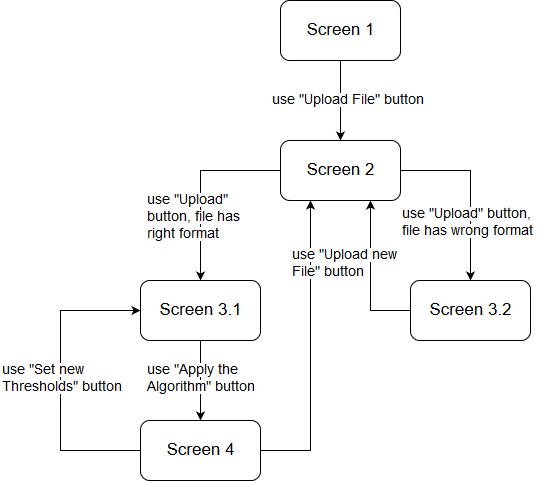
\includegraphics[scale=0.7]{ScreenFlow.png}

\subsubsection{Screen 1}

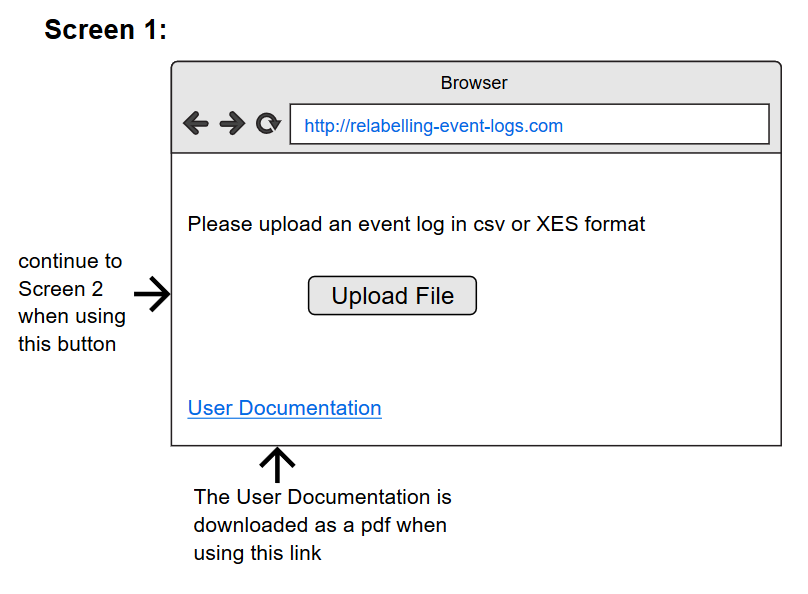
\includegraphics[scale=0.8]{InterfaceMockup1.png}


The first screen visible to the user will show a description saying that an event log in CSV of XES format should be uploaded. Moreover, a button ``Upload File" is visible. By using this button, the user will continue to Screen 2. At the end of the page, there will be a link called ``User Documentation". By clicking on this link, the User Documentation will be downloaded in pdf format.
\subsubsection{Screen 2}

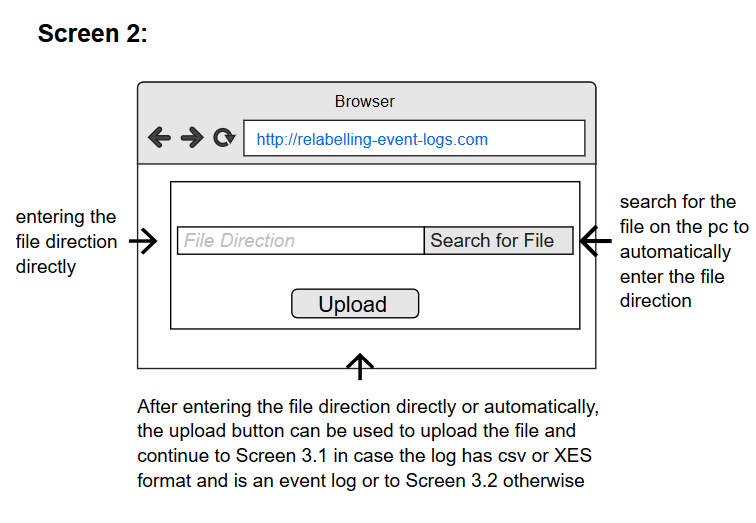
\includegraphics[scale=0.9]{InterfaceMockup2.png}

In the second screen visible to the user, the user can enter the file direction of the event log he wants to upload. He can either directly type in the direction into the ``File Direction" field or use the ``search for File" button to search for a file on his PC, so that the direction will automatically be filled in after selecting a file.

After using one of this alternatives, he can use the ``Upload" button to upload the file with the given directory. In case this file is an event log, i.e., the data contains at least the attributes ``id", ``time stamp" and ``activity name", and has either CSV or XES format, the user will continue to Screen 3.1. If one of these conditions is not satisfied, he will continue to Screen 3.2. 


\subsubsection{Screen 3.1}
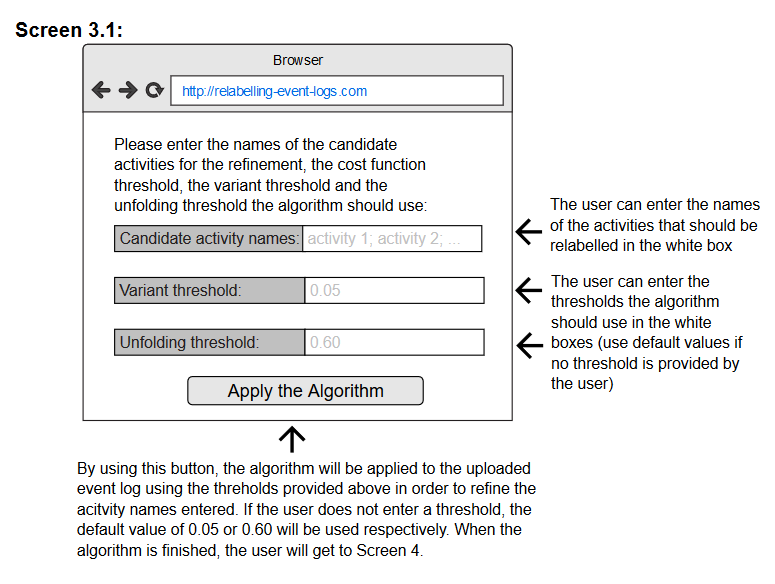
\includegraphics[scale=0.9]{InterfaceMockup3-1.png}

This screen appears if the file uploaded by the user meets the requirements. In this screen, the user can set the candidate activity names, i.e., those activities that the algorithm can relabel. Moreover, the user can set the thresholds for the algorithm, i.e., the variant and the unfolding threshold. He can enter all of these in the corresponding white boxes. If he does not enter the thresholds, the default values of 0.05 and 0.60 will be used respectively. Using the button ``Apply the Algorithm", the web service will start applying the algorithm using the provided thresholds. After the algorithm is finished, the user will get to Screen 4.

\subsubsection{Screen 3.2}
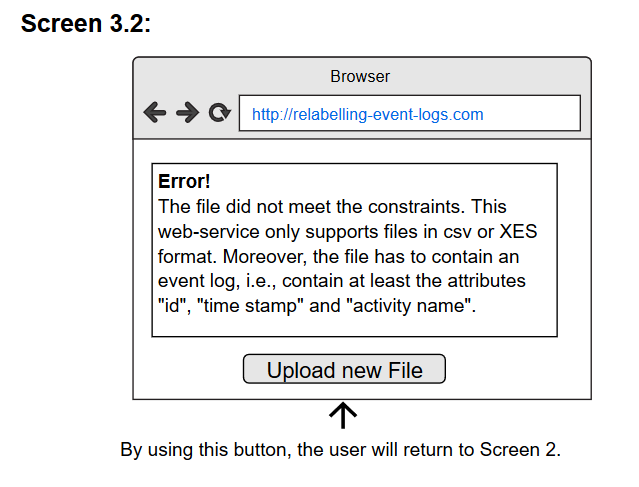
\includegraphics[scale=0.9]{InterfaceMockup3-2.png}

This screen appears if the upload was not successful because the file did not meet the assumptions. If the file does not have the right format, the user can click on the button ``Upload new File" to return to Screen 2 and upload a file that meets the constraints.


\subsubsection{Screen 4}
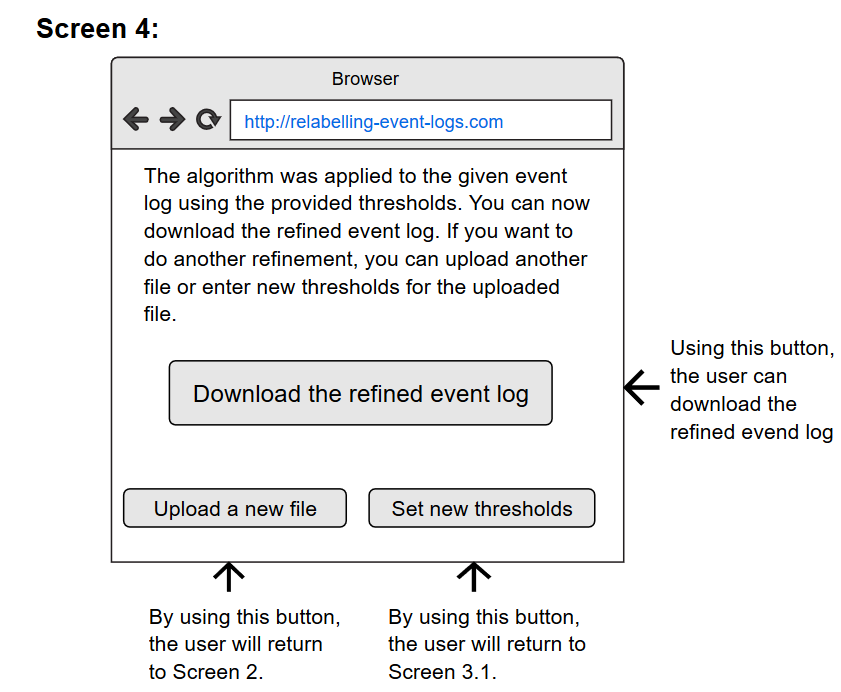
\includegraphics[scale=0.8]{InterfaceMockup4.png}

This Screen will be shown after finishing the algorithm. The user can now download the refined log using the corresponding button. After this step, the user is done and can exit the page, but if he also wants to apply the algorithm to another event log or to the same event log using different thresholds, he can use the corresponding buttons and will be redirected to Screen 2 or Screen 3.1 respectively.


%\newpage
%\bibliographystyle{plain}
%\bibliography{references}  




%\addcontentsline{toc}{chapter}{\textbf{References}}
\end{flushleft}
%\bibliography{uw-ethesis}
% Tip 5: You can create multiple .bib files to organize your references. 
% Just list them all in the \bibliogaphy command, separated by commas (no spaces).

% The following statement causes the specified references to be added to the bibliography% even if they were not 
% cited in the text. The asterisk is a wildcard that causes all entries in the bibliographic database to be included (optional).


\begin{thebibliography}{5}
\bibitem{paper}
Lu, Xixi, et al. ``Handling duplicated tasks in process discovery by refining event labels." International Conference on Business Process Management. Springer, Cham, 2016.

\bibitem{matchings}
Xixi Lu1, Dirk Fahland, Frank J.H.M. van den Biggelaar, Wil M.P. van der Aalst. ``Detecting Deviating Behaviors without Models."


\end{thebibliography}










\end{document}
